Historically programs or applications run locally on a client device such as a personal computer. Since the introduction of the iPhone in 2007 and the release of the iOS app store in 2008 followed by the introduction of Google Play later the same year many %use numbers here?
has gotten acquainted with mobile apps, applications that run locally on a mobile device.

A web app is a interactive web site where content are read and written to pages dynamically based on various type of input, including input from usage of mouse and keyboard.

The last few years the web has evolved from simply being a platform for websites to also be a platform for web apps. Web applications, or web apps for short, is a type of application that run inside a web browser. Traditionally web applications a built with a thin user interface layer through which the user interacted with the application, while the actual computation was executed on one or more servers, % in the cloud
passing data back and forth between the client and the server.

Web apps are based on HTML, CSS, and JavaScript \parencite{ParkJungMoon2015}, the same web technologies originally conceived to share documents. JavaScript was a major addition to the set of web technologies as web apps are made possible through use of JavaScript \parencite{ParkJungMoon2015}. JavaScript is increasingly popular for building high performance apps \parencite{SandhuHerreraHendren2018}. As modern devices becomes increasingly more powerful, more and more web apps are built to do computing client side.

\begin{comment}

\hl{TODO: reference }
Figure \ref{google-docs}
    
\begin{figure}[!h]
\centering
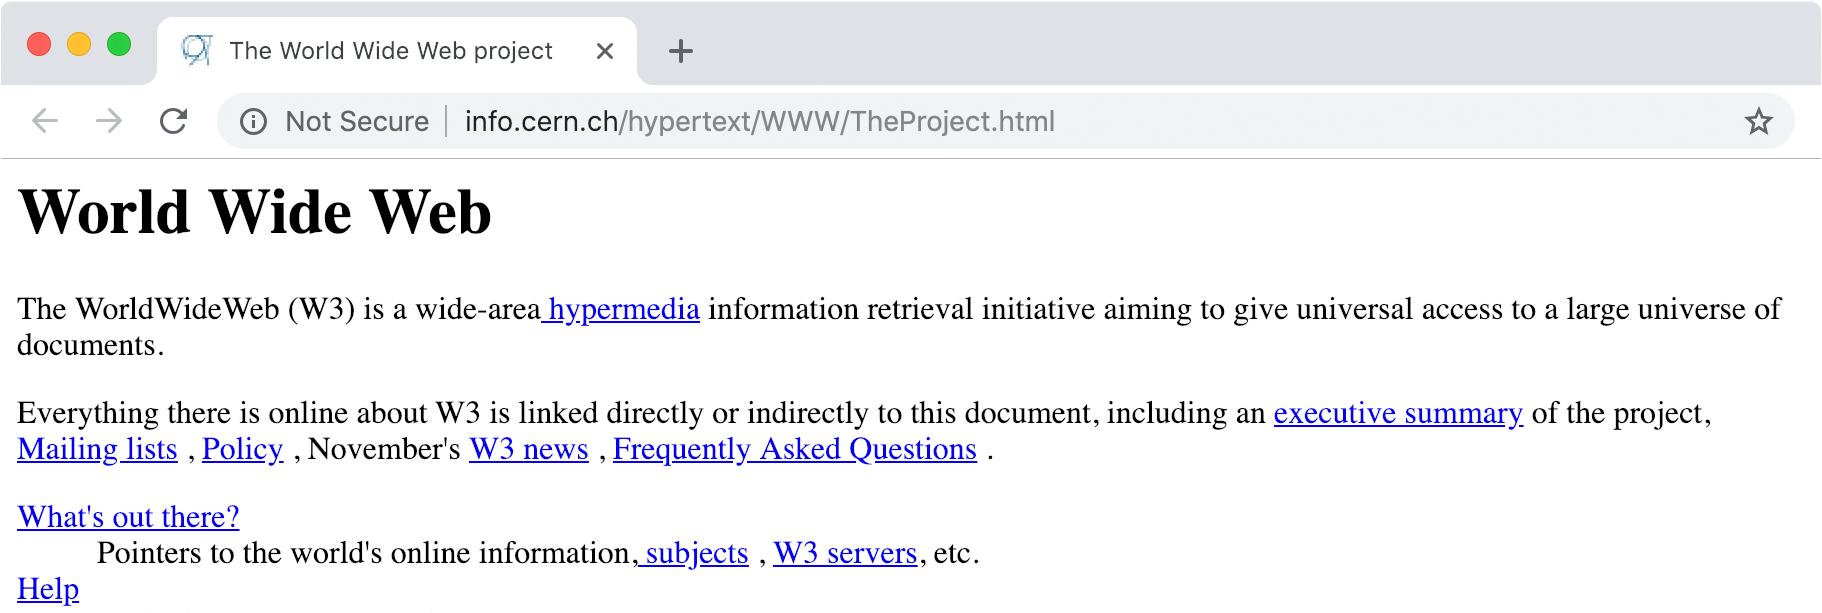
\includegraphics[width=16cm,keepaspectratio]{../Figures/world-wide-web}
\caption{The first web page created by Tim Berners-Lee.}
\label{world-wide-web}
\end{figure}

\begin{figure}[!h]
\centering
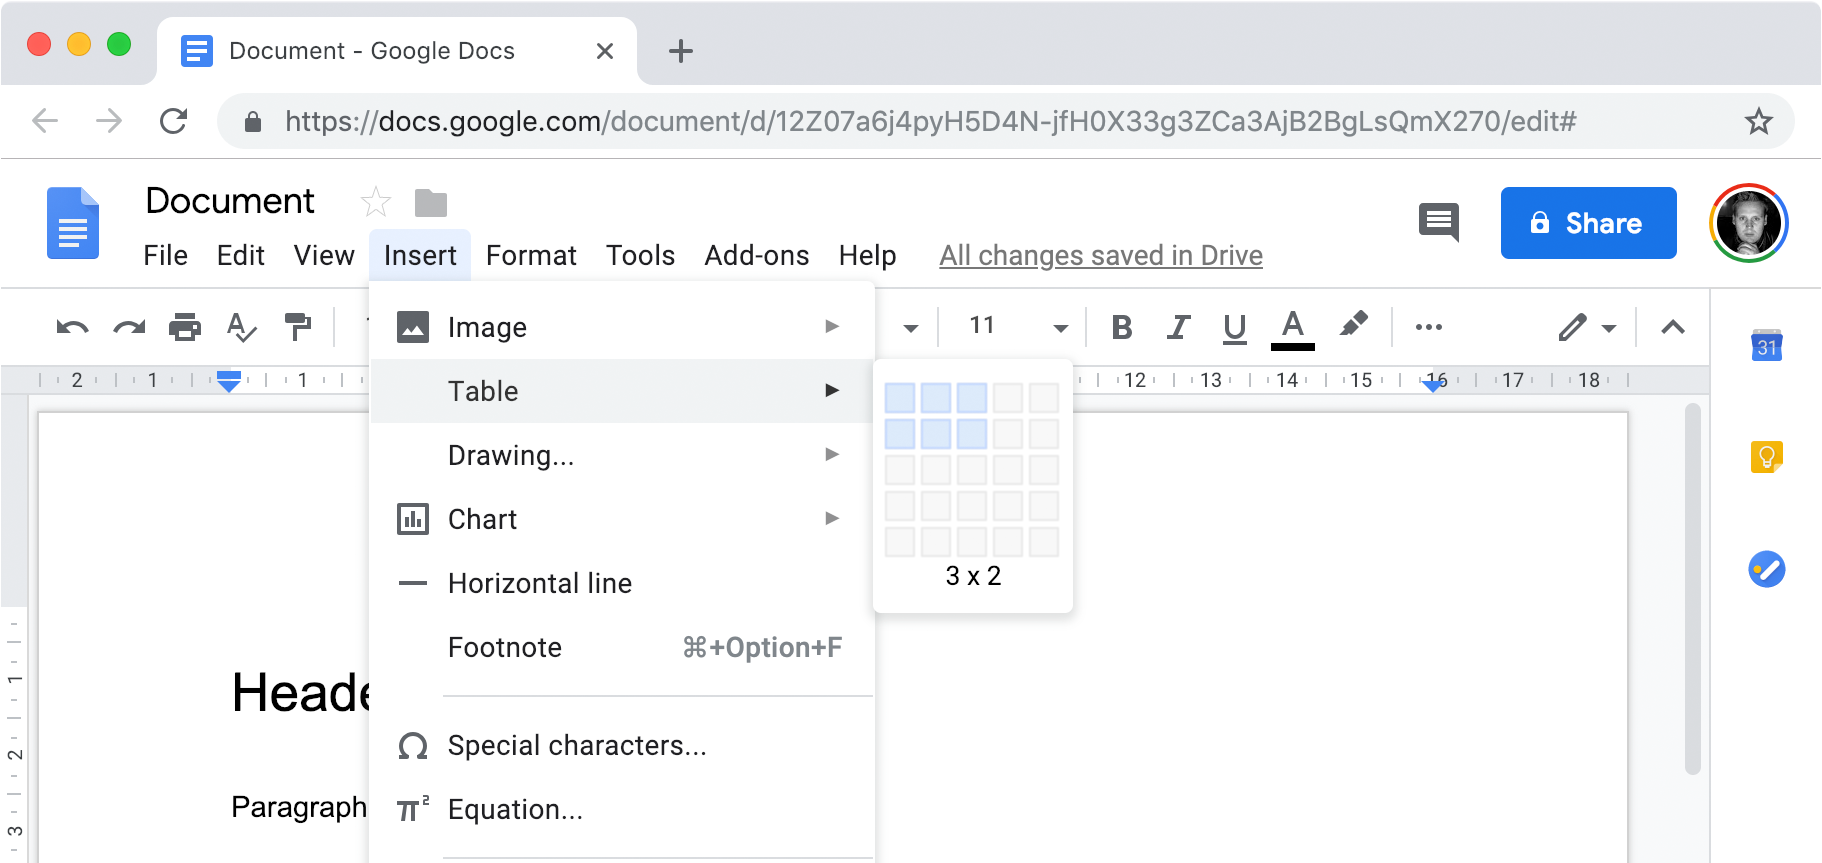
\includegraphics[width=16cm,keepaspectratio]{../Figures/google-docs}
\caption{Google Docs is a modern web application that enables users to run an office suite in a web browser.}
\label{google-docs}
\end{figure}

\end{comment}
